\documentclass[12pt,a4paper]{paper}
\usepackage[latin5]{inputenc}
\usepackage[T1]{fontenc}
\usepackage{graphicx}
\usepackage{amsmath, amssymb}
\usepackage{listings}
\usepackage{verbatim}
\usepackage{rotating}
\graphicspath{{images/}} % Graphics will be here
\usepackage{listings}
\usepackage{float}
\usepackage{perpage}
\usepackage{setspace}

\onehalfspacing
\parskip 7.2pt 
\MakeSorted{figure}
\MakeSorted{table}

\title{WEB BASED SIMULATION GAME DEVELOPMENT SOFTWARE: MASHAP}
\author{Mert Nuhoglu\\
	Bogazici University,
	Istanbul, Turkey\\
	\texttt{mert.nuhoglu@gmail.com}
}
\date{\today}

\begin{document}
\lstset{
         basicstyle=\footnotesize\ttfamily, % Standardschrift
         numberstyle=\tiny,          % Stil der Zeilennummern
         numbersep=5pt,              % Abstand der Nummern zum Text
         tabsize=2,                  % Groesse von Tabs
         extendedchars=true,         %
         breaklines=true,            % Zeilen werden Umgebrochen
%         keywordstyle=\color{red},
                frame=b,         
%         stringstyle=\color{blue}\ttfamily, % Farbe der String
         showspaces=false,           % Leerzeichen anzeigen ?
         showtabs=false,             % Tabs anzeigen ?
         xleftmargin=0pt,
         framexleftmargin=0pt,
         framexrightmargin=0pt,
         framexbottommargin=4pt,
         showstringspaces=false,     % Leerzeichen in Strings anzeigen ?
         escapeinside={(*}{*)},
%         literate={\_}{}{0\discretionary{\_}{}{\_}}
				 literate={\_}{\_}{1},
				 frame=tb 									 % horizontal line above
}

\pagenumbering{roman}

\maketitle

\begin{abstract}
System Dynamics researchers need a software tool that makes the simulation games easy to access through web user interface. We developed a software (Mashap) that automatically generates and runs a web based simulation game for any system dynamics model. Our software has some important advantages over the existing ones: First, it is an open platform on which new tools can be built. Second, it is built for generating web games for all system dynamics modeling software. Mashap enables the system dynamics researchers to build web based gaming environments for their own models. The purpose of this paper is to introduce you to Mashap. To do this, I will show in detail how to use Mashap to develop a web based game for a body weight dynamics model. 
\end{abstract}

\section{Introduction}

The aim of this paper is to introduce Mashap to the system dynamics community. Mashap is a web application that produces and runs simulation games for system dynamics models. The application is designed to run any system dynamics model developed in popular model building tools such as Vensim or Stella. 

The game engine, called Mashap, is able to generate web user interfaces and run any system dynamics model developed in Vensim, currently. Support for other software can be added easily to Mashap. The aim of the tool is to provide a web based game building environment for system dynamics researchers around the world.

Currently, there are several software that run system dynamics simulation models on the web, but current software have several constraints that necessitate development of new tools. The primary constraint of the current software is that they are commercially licensed, closed source products. This is a hinder to building new tools upon the current ones. Open source or free software allows people to build innovative tools upon existing software that the original programmers could not imagine or afford on their own. This need is the fundamental rationale for the development of the general web based game engine in this research.

Currently, Mashap supports only Vensim and Mapsys as input files. Support for Stella and Powersim are planned. Mashap can run simulation by itself and it can build a gaming environment for simulation models automatically. There are several popular software in system dynamics domain: Stella (and Netsim upon it), Vensim, Powersim, and Forio.

Mashap is designed as a complementary tool to the current, popular model development tools not as a directly competing tool. In terms of supported features, Mashap is far ulterior than these four tools. But Mashap has some unique features that can make Mashap useful in some use cases:

The cost of development of a web based simulation game is much lower in Mashap than all of the four software when having a simple, automatically generated user interface for a game is enough. The server side software Netsim has very high price. Powersim and Vensim are cheaper in terms of price but they don't support web interfaces out of the box. 

Web user interface development is much easier in Mashap than Forio. Forio has many features that allow the game developers to customize the user interface finely. Netsim is very easy to use too. It does not require the model builder to develop web interface in a special language. Netsim builds a flash based web user interface from a game developed in Stella.

Primary constraint of current software is that they are commercially licensed, closed source products. Commercial licensing is a hinder on the universal access to software. But there are much more important, implicit consequences of closed source software. Closed source software prevent people to build new tools based on current software seriously. This is actually more important than access to software. Most software tools are pretty cheap today. It is easy to find the funds to buy them. But building something new upon existing software is the real burden of closed source software.

Normally this might not be a problem if the domain space of the requirements of the users were explored extensively. But in science communities this is rarely possible. Scientific research extends to new frontiers continuously. It is crucial that new tools are developed in parallel to research.

Open source or free software allows the people to build very innovative tools upon existing software that the original programmers could not imagine or afford on their own. This need is the fundamental rationale for development of a general web based game engine in this research.
	
% rationale
\section{Rationale}

Mashap can produce web based, simulation games for any system dynamics model. Mashap produces the web based game automatically without requiring any additional work. We expect that system dynamics researchers will use Mashap to build web gaming environments for their own models.

Web based games have several important advantages over desktop games:

\begin{enumerate}
	\item Access to general public is much easier for web applications. Anyone who has access to a browser can play the game.
	\item Access to domain experts for validation, testing, dissemination, or model development is much easier.
	\item Maintenance of the software is much less costly for programmers. There is no burden for updates, patches, or support for different operating systems.
\end{enumerate}

An additional benefit of web based game engine Mashap is that it can become a base for group modeling. We assume that having effective tools for group modeling is crucial for group modeling to realize its actual potential. Current software are not designed for collaborative model development. Desktop software is not suitable for collaboration by its nature. Mashap is not developed for collaboration either, but it is possible to build collaborative features upon Mashap.

\section{User Requirements}

There are two distinct types of users for Mashap:

\begin{itemize}
	\item Model builders
	\item Game players
\end{itemize}

Model builders and game players have different goals. We assumed that model builders have the following goals and expectations in using a web based game engine like Mashap:

\begin{itemize}
	\item To make the simulation available to a lot of people easily
	\item To continue using their accustomed tools such as Vensim or Stella for model building
	\item To verify the correctness of the simulations
	\item To get the web game up instantly without spending a lot of labor for customization or configuration of the software
	\item To access to the run data of the games of the end users
	\item To experiment the same model with different parameters or other factors
\end{itemize}

We assumed that game players have the following goals and expectations in using a web based simulation game built upon Mashap:

\begin{itemize}
	\item To see the effects of their decisions instantly
	\item To get convinced of the validity of the game
	\item To learn something about a complex system or to develop an effective strategy to deal with the problems
	\item To see effects of their current behavior in long term
	\item To socialize over games
\end{itemize}

The first four goals are actually valid for any system dynamics game, not only for web games. To socialize over games is a goal specific to web games. Now, people play games not only for the enjoyment they get from the game itself; many popular games have some kind of socializing feature. Game players like to compare themselves with other people or to enjoy playing games together with their friends. Mashap currently does not have any feature to satisfy socialization requirements, but it has the infrastructure to support socialization features.

\section{Design}

The application has three basic features:

\begin{enumerate}
	\item Conversion of models built in a system dynamics modeling software into Python syntax
	\item Running simulation of system dynamics models
	\item Automatic user interface generation to construct web simulation games
\end{enumerate}

The system currently supports conversion of Vensim files into Python format. Support for import from Mapsys and export to Matlab and Excel are partially completed. Support for import from Stella and Powersim model files are planned.

Simulation of system dynamics models are done by a numerical integration solver implementing 4th order Runge-Kutta method for solving the initial value problem $\frac{d\vec{y}}{dt}=F(t,\vec{y})$ and $\vec{y}(0)=\vec{\alpha}$.

Automatic generation of web user interface of the game is done according to the decisions made by the model builder in the preparation of the game. The model builder gives the system three decisions as input:

\begin{enumerate}
	\item Initial parameters: The variables of the model that will be initialized at the beginning of the game
	\item Decision variables: The variables that will be fed into the system
	\item Output groups: The outputs of the model at each decision step to be produced by the system
\end{enumerate}

The system builds the game user interface according to these three decisions automatically.

\subsection{Assumptions and Dependencies}

There are several assumptions that guided the design decisions of Mashap:

\begin{enumerate}
	\item Model builders won't prefer to learn another model development tool instead of the popular software such as Vensim or Stella. 
	\item Model builders won't prefer to learn any special language or configuration format for game preparation.
	\item Game players will possibly prefer to enter their decisions inside the game in various ways such as by a batch file prepared in Excel or by some convenient graphical tools.
	\item Some modules of Mashap can possibly be used as an infrastructure for development of other software in some domains such as modeling, gaming, or validating.
	\item The simulation engine of Mashap can possibly be transferred to client side due to capacity limits of server's computing power.
\end{enumerate}

One of the primary assumptions under the design decisions of Mashap is that model builders are accustomed to their current model development tools strongly and they would't prefer to learn another tool doing the same job in a different way. Therefore, we do not try to imitate any core functionalities of model development tools such as Vensim or Stella. Another implication of this assumption is that model builders won't like to enter the equations of the model by hand or any other method. They would like to use their current model building environment. Mashap will be used as a complementary tool that is going to be used for purposes that are not currently handled by popular software in an easy or standard way.

Another assumption about preferences of model builders is that they won't prefer to learn any special language or a cumbersome configuration format when preparing a game environment from their models. Forio is probably the mostly used software for web based simulation games in system dynamics domain. Forio requires the model builders to prepare the game by using a special language. This feature allows a lot of flexibility for the customization of the game user interface. We don't have any solid, empirical proof for our argument, but we assumed that usability is more important than flexibility.

Another assumption is that game players will possibly prefer to enter their decisions inside the game in various ways such as by a batch file prepared in Excel or by some convenient graphical tools. Web applications do not have the same interactivity level as desktop applications. Gaming environments prepared with Stella or Vensim has a lot of interaction with the game player. In web environment, the waiting time from submitting a decision until taking the response is so long that the users cannot get into the same flow of interaction as in desktop applications. Therefore, we assumed that the interaction between the user and the software can evolve to new methods. An alternative for the interaction method is entering the decisions as a batch in one step or in a few steps for the duration of simulation's run time. The batch data can be entered with an Excel file or it can be produced by the user on an interactive graphics that lies on the web application.

An assumption on the development of Mashap is that some modules of Mashap can possibly be used as an infrastructure for development of other software. Mashap is released under a free software license. Other programmers can extend the software for their own purposes. We guess that a group modeling tool in the style of social web applications or a tool that helps the researcher to perform an experiment with different parameters in a model can be built upon Mashap.

The assumptions above are all related to the possible changes in functionality of Mashap. There are some possible changes that involve the architecture of the software as well. One of them is that there can be severe capacity problems in the servers' computing power where Mashap is hosted because simulation requires a lot of computing power. The capacity problem might necessitate the transfer of the simulation engine from the server side to the client side. Therefore the architecture of Mashap should be decomposable into independently working modules. A simulation engine running on the web browser (client side), which is probably implemented in Javascript, should be able to communicate with Mashap's server components seamlessly.

\subsection{System Architecture}

Figure~\ref{fig:layers} shows the layers of the system architecture of Mashap. This diagram shows the core modules of Mashap. It does not include noncritical modules or external modules. Each box denotes one layer of the architecture. The modules that constitute the layer are put inside the box. The directed associations between the modules and layers denote the dependencies between them. The dependency of presentation layer on domain model is exceptional; therefore it is drawn as a dashed association. \\ 

\begin{figure}
	\centering
	\fbox{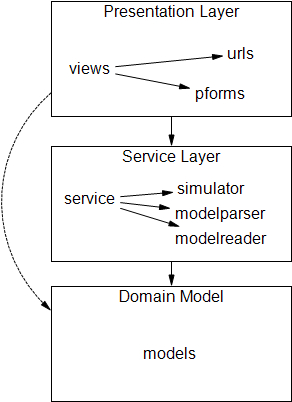
\includegraphics[scale=0.5]{807}}
\caption{Layers of the system architecture of Mashap}%
\label{fig:layers}%
\end{figure}

The application consists of three basic layers. Presentation layer is responsible for everything related to the user interface such as presenting information to the user and getting user commands. Service layer is responsible for coordinating the business logic. It also contains processing logic that does not fit into domain objects such as performing the simulation or converting the model files from Vensim format to Python format. Domain model contains information about the domain. This is the core of the software. The state of the business objects is held here.

Presentation layer consists of three core modules: views, urls, and pforms. The module views is a thin layer that delegates the input received from the user to the service layer and prepares the user interface that user gets. The module views delegates actual preparation of the user interface to pforms module and html templates. The module pforms produces form components in html pages. Form components consist of form widgets such as combo boxes or text boxes. The module pforms is responsible for checking submitted data against a set of validation rules and converting form data to the corresponding Python data types. The module urls is responsible for navigating between the web pages and views functions.

Nearly, every views function correspond to a web page. A views function consists of two parts: get and post. The post part is responsible for receiving the input of the user and delegating the control to the service layer. The get part is responsible for making the user interface, that the user will see, with the help of pforms module.

Service layer consists of four core modules and some small helper modules. The module service is a thin layer that is responsible for coordinating the business logic. It performs this with the help of the other three modules. The module simulator is responsible for performing the simulation. It delegates numerical integration to the helper module "run\_kut4". The module modelreader reads a list of equations expressing a system dynamics model in Python syntax. The module reads the equations and builds the domain objects ModelPython and ModelDefinition. The module modelparser parses and converts a model file of Vensim into a list of equations in Python syntax.

Domain model consists of one module: models. The module models contains the definitions of the domain model objects shown in \ref{fig:domain_model}. \\

\begin{figure}
	\centering
	\fbox{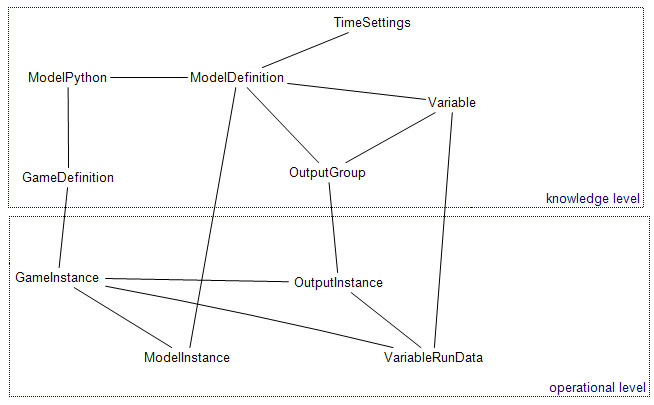
\includegraphics[width=\columnwidth]{808}}
\caption{Domain model of the Mashap software}%
\label{fig:domain_model}%
\end{figure}

\paragraph{Topological ordering of equations}
The equations in Vensim's model file are in an arbitrary order. This is not suitable for simulation algorithm because the simulation algorithm advance step by step for each variable. All the dependent terms of a variable must be calculated before calculating the variable itself. Therefore the equations must be fed into the simulation algorithm in the order of dependencies. The ordering is done with the topological sorting algorithm. 

\paragraph{Usage of dynamic forms}
The user interface of the game is produced  automatically according to the decisions made by the model builder in the preparation of the game. The model builder gives the system three inputs: initial variables, decision variables, output groups. The system generates a dynamic user interface according to these choices. This functionality is the responsibility of pforms module.

\section{Usage}

Mashap is designed to produce web based, interactive dynamic system simulation games for any system dynamics model. As the proof of concept application, we use Mashap to develop a web based game for the body weight dynamics model. The example game is called Body Weight Websim. The aim of Body Weight Websim is to allow users to explore the possible effects of nutrition and physical exercising on the long term dynamics of body weight of the human realistically. The model beneath Body Weight Websim is a modified version of Hall's body weight simulation model \cite{Hall2006}.

Mashap produces the web based game instantly from the input Vensim file that holds body weight dynamics model without requiring any additional work except entering decisions required for the customization of game user interface. The relationship between Vensim model file, Mashap, and Body Weight Websim is shown in Figure~\ref{fig:mashap_and_body_weight_websim}. The model builder inputs her decisions to customize the game interface. Mashap produces from these inputs the Body Weight Websim game. The game players access to the Body Weight Websim game. \\ 

\begin{figure}
	\centering
	\fbox{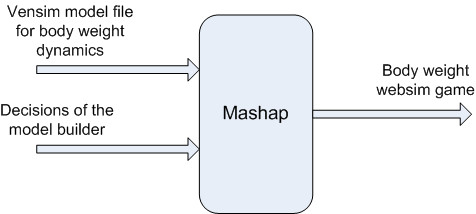
\includegraphics[scale=0.5]{809}}
\caption{The relationship between Vensim model file, Mashap, and Body Weight Websim game}%
\label{fig:mashap_and_body_weight_websim}%
\end{figure}

Mashap is a platform that is designed to host several websim games at the same time as shown in Figure~\ref{fig:mashap_platform_hosts_many_games}. Also model builder can produce as many different versions from the same model file as she wishes. The Figure~\ref{fig:mashap_platform_hosts_many_games} shows that there are two versions of Body Weight Websim. Anytime the user inputs a different Vensim model file or set of decisions that customize the game, Mashap produces a new version of the game. This feature allows the researchers to experiment a simulation model with different sets of parameters.

Mashap produces a unique address for each game. Anybody who knows the address of the game can access and play the game. When a researcher designs an experiment with different sets of parameters, she can disseminate different url addresses for different versions of the same game to different sample groups. \\ 

\begin{figure}
	\centering
	\fbox{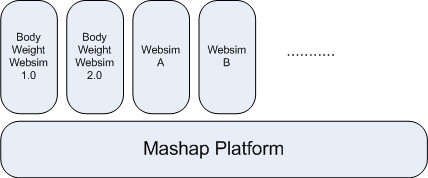
\includegraphics[scale=0.5]{810}}
\caption{Mashap is a platform that can host several websim games.}%
\label{fig:mashap_platform_hosts_many_games}%
\end{figure}

To prepare the Body Weight Websim game on Mashap, the model builder inputs four different types of decisions:

\begin{enumerate}
	\item Initial parameters 
	\item Decision variables 
	\item Output groups 
	\item Time settings 
\end{enumerate}

In Body Weight Websim, initial parameters let the model adapt itself to the specific metabolic characteristics of the simulated person from whom the initial parameters are taken. The selection of initial parameters is a critical decision that depends on the model at hand. The model has to be designed taking the initial parameters into consideration because initial parameters can effect the initialization of stocks and several characteristic features of the model. 

The decision variables are the parameters of which values the game player assigns at every game step. The game player manages the system under the game by using the decision variables. 

An output group consists of a group of variables. Mashap draws the graphics of the dynamics of the variables put into output groups during simulation at every game step.

Time settings consist of time related settings of the simulation. There are four such settings in Mashap: time between decision steps, time step, total game time, and record period. Time between decision steps is the length of the simulation time between two consecutive game steps. Time step is the size of $dt$ used in numerical integration algorithm. This value does not have any real life meaning. Total game time is the length of the game in simulation time. Record period is the length of time between two points where Mashap records the values of the variables in output groups into the database.

The user interface of the Body Weight Websim that the game player interacts with is shown in Figure~\ref{fig:user_interface_for_game_player}. This user interface is automatically generated by Mashap after getting the inputs (initial parameters, decision variables, output groups, time settings) from the model builder.

\begin{figure}
	\centering
	\fbox{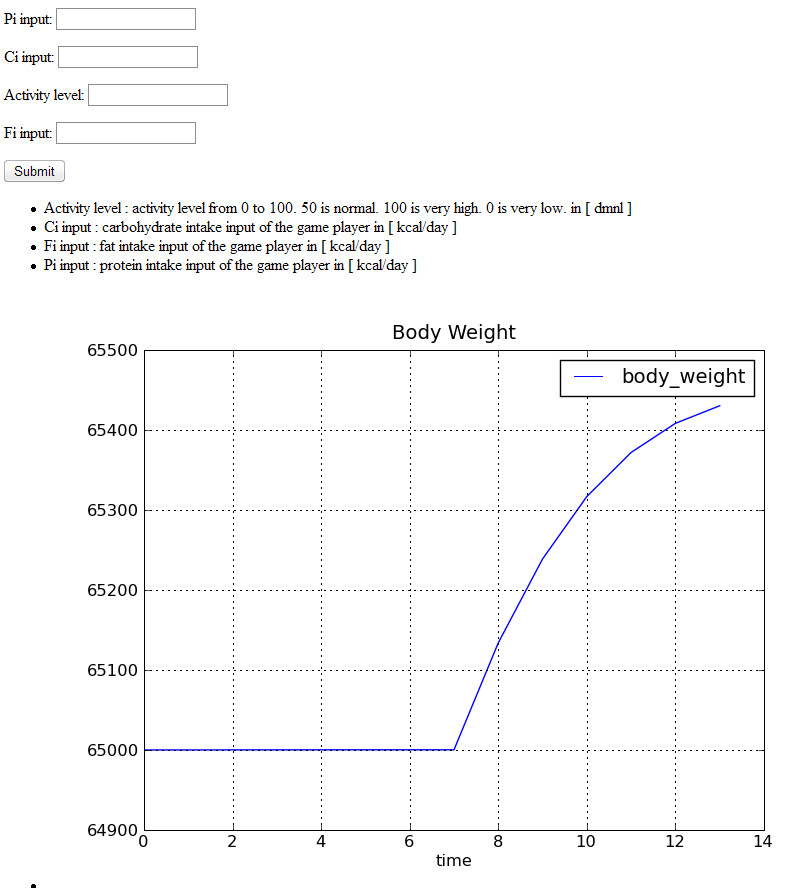
\includegraphics[scale=0.6]{895}}
\caption{User interface of the Body Weight Websim}%
\label{fig:user_interface_for_game_player}%
\end{figure}

\section{Conclusion}
Mashap is designed to run any system dynamics model developed in popular model building tools such as Vensim or Stella. Mashap can produce web based, simulation games from any system dynamics model automatically without requiring any additional work for configuration.

There are two important use cases for Mashap. First, model builder uploads the model and prepares the game. Second, a user/player plays the game. In preparation of the game, the model builder specifies four different sets of decisions: initial parameters, decision variables, output groups, and time settings. Mashap customizes and produces the user interface of the game by using these inputs. Body Weight Websim is an example game built with Mashap. 

There may be several improvement areas for Mashap. The support for Stella, Powersim model files can be added. The partial capability of exporting of the model's equations to Matlab format can be completed. There are several improvement potentials in the usability of the software. Data entry can be made through more convenient ways such as by uploading an Excel file or by using a graphical tool.

Scalability of Mashap is one of the important technical requirements. To achieve higher scalability without incurring high amounts of server costs, there are some solution alternatives: transferring the simulation engine to the client side and using a non-relational database such as Google's BigTable.

Lastly, the software can be improved by implementing innovative, collaborative use cases. Current popular, modeling and simulation software are not designed for collaborative model development. Mashap can serve as a platform for developing collaborative tools upon it.

The code of the Mashap software is available from \lstinline|http://code.google.com/p/mashap/|. Working Mashap software is live on \lstinline|http://sesdyn.ie.boun.edu.tr/mashap/|.

\begin{thebibliography}{99}

    \bibitem{Hall2006} Hall KD. ``Computational model of in vivo human energy metabolism during semistarvation and refeeding". \textit{Am J Physiol Endocrinol Metab}, Vol~291(1), July 2006.

\end{thebibliography}

\end{document}
